%%%%%%%%%%%%%%%%%%%%%%%%%%%%%%%%%%%%%%%%%%%%%%%%%%%%%%%%%%%%%%%%%%%%%%%%%%%%%%
%%%%%%%%%%%%%%%%%%%%%%%%%%%%%%%%%%%%%%%%%%%%%%%%%%%%%%%%%%%%%%%%%%%%%%%%%%%%%%
%%
%% Dokumentacia k semestralnemu projektu z PRL
%%
%%%%%%%%%%%%%%%%%%%%%%%%%%%%%%%%%%%%%%%%%%%%%%%%%%%%%%%%%%%%%%%%%%%%%%%%%%%%%%
%%%%%%%%%%%%%%%%%%%%%%%%%%%%%%%%%%%%%%%%%%%%%%%%%%%%%%%%%%%%%%%%%%%%%%%%%%%%%%
\documentclass[12pt,a4paper,titlepage,final]{article}

% cestina a fonty
\usepackage[czech]{babel}
\usepackage[T1]{fontenc}
\usepackage[utf8]{inputenc}
% balicky pro odkazy
\usepackage[bookmarksopen,colorlinks,plainpages=false,urlcolor=blue,unicode]{hyperref}
\usepackage{url}
% obrazky
\usepackage[dvipdf]{graphicx}
% velikost stranky
\usepackage[top=3.5cm, left=2.5cm, text={17cm, 24cm}, ignorefoot]{geometry}

\begin{document}

%%%%%%%%%%%%%%%%%%%%%%%%%%%%%%%%%%%%%%%%%%%%%%%%%%%%%%%%%%%%%%%%%%%%%%%%%%%%%%
% titulná strana

% !!!!!!!!!!!!!!!!!!!!!!!!!!!!!!!!!!!!!!!!!!!!!!!!!
\def\projname{Projekt z predmetu PRL \\ Implementácie algoritmu Minimum extraction sort}
% !!!!!!!!!!!!!!!!!!!!!!!!!!!!!!!!!!!!!!!!!!!!!!!!!



\title{Implementácia algoritmu Minimum Extraction sort}
\date{Marec 31 2016}
\author{Martin Maga (xmagam00)}
\maketitle

\section{Teoretické rozobratie algoritmu}
Algoritmus pracuje nad binárním stromem, v jehož listech jsou na počátku uloženy řazené hodnoty.
Všechny nelistové uzly obsahují procesor, který je schopen porovnat hodnoty potomků a menší z nich
uložit do svého uzlu. Hodnota menšího z potomků se tedy posunuje stromem vzhůru, až dosáhne
kořene – po (log n) + 1 krocích. Následně do kořenového uzlu postupují další nejnižší hodnoty – vždy
ve dvou krocích – nejprve se hodnota dostane do kořene, a pak je z ní odstraněna do pole
s výsledkem. Jde o binární strom, tzn. počet listů je vždy mocninou dvojky. Abychom mohli řadit i
hodnoty, jejichž počet není mocninou dvojky, musíme si u zbývajících listů poznamenat, že jsou
prázdné. U každého uzlu si tedy pamatujeme hodnotu, kterou obsahuje, a také proměnnou, ve které
uchováváme (ne)prázdnost uzlu.

\section{Teoretická časová zložitosť}
Nejmenší hodnota dosáhne kořene stromu po (log n) + 1 kroku. Následně je zbývajících n – 1 hodnot
ze stromu „odstraněno“ v pořadí od nejmenší vždy po dvou krocích – prvním je doručení hodnoty do
kořene, druhým je odstranění hodnoty z kořene a uložení do výsledného pole.
Celkový počet kroků je tedy 2 * (n – 1) + (log n) + 1 = 2 * n + log n – 1. Dominantní složkou složitosti je
n, jde tedy o algoritmus s lineární časovou složitostí.


\subsection{Problémy pri snímaní}
V prípade snímania mydla sme po nanesení na prst museli mydlo jemne zotrieť, pretože snímač nebol opakovanie schopný zosnímať odtlačok. Čo sa týka druhého detergentu oleja, tak po nanesení bol odtlačok ihneď rozoznaný. Často sa vyskytla aj situácia pokiaľ osoba mala prst mastný, tak snímač skôr rozoznal odtlačok ako pri suchom a čistom prste. Rovnako sme narazili, že studené prsty ľudí, ktorí práve prišli z vonká bolo nasnímanie rýchlejšie ako ľudí, ktorí sa už nejaký čas nachádzali vo vnútri v teple.

Pri niektorých osobách sa nám nepodarilo získať niektoré odtlačky. Hlavne sa jednalo o staršie osoby z našej skupiny, ktorých papilárne línie neboli výrazné (mierne poničené), resp od ľudí, ktorí pracujú z chemických prostriedkami, ktoré spôsobujú poškodzovanie papilárnych línií.


\section{Vyhodnotenie odtlačkov prstov s olejom}
V nasledujúcej kapitole pojednávame o otiskoch prstoch, na ktoré bol aplikovaný olej. Vybrali sme nasledujúce odtlačky prstov, na ktorých je najlepšie viditeľný vplyv oleja. Vplyv oleja je badateľný na papilárnych líniach, ktoré sú stenšené a viditelnejšie. Ako referenčný prst sme použili prostredník ľavej ruky.

\begin{center}Odtlačky s olejom \end{center}
\begin{figure}[h]
  \centering
  \begin{minipage}[b]{0.20\textwidth}
    \scalebox{0.5}{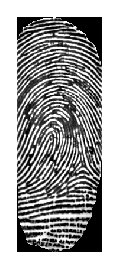
\includegraphics[width=\textwidth]{img/44_L3_3_2.eps}}
    
  \end{minipage}
  \hfill
  \begin{minipage}[b]{0.20\textwidth}
    \scalebox{0.5}{
\includegraphics[width=\textwidth]{img/6_L3_3_2.eps}}
    
  \end{minipage}
  \hfill
  \begin{minipage}[b]{0.20\textwidth}
    \scalebox{0.5}{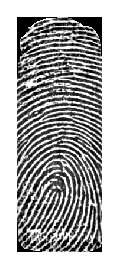
\includegraphics[width=\textwidth]{img/12_L3_3_2.eps}}
    
  \end{minipage}
  \hfill
  \begin{minipage}[b]{0.20\textwidth}
    \scalebox{0.5}{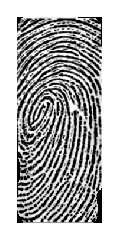
\includegraphics[width=\textwidth]{img/35_L3_3_2.eps}}
    
  \end{minipage}
\end{figure}
\begin{center}Odtlačky bez oleja \end{center}
\begin{figure}[h]
  \centering
  \begin{minipage}[b]{0.2\textwidth}
    \scalebox{0.6}{
\includegraphics[width=\textwidth]{img/42_L3_3_1.eps}}
    \label{Osoba 1}
  \end{minipage}
  \hfill
  \begin{minipage}[b]{0.2\textwidth}
    \scalebox{0.5}{
\includegraphics[width=\textwidth]{img/4_L3_3_2.eps}}
    \label{Osoba 2}
  \end{minipage}
  \hfill
  \begin{minipage}[b]{0.2\textwidth}
    \scalebox{0.5}{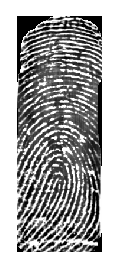
\includegraphics[width=\textwidth]{img/10_L3_3_2.eps}}
    
    \label{Osoba 3}
  \end{minipage}
  \hfill
  \begin{minipage}[b]{0.2\textwidth}
    \scalebox{0.5}{
\includegraphics[width=\textwidth]{img/33_L3_3_1.eps}}
    \label{Osoba 4}
  \end{minipage}
\end{figure}

Odtlačky prstu na 1. obrázku zľava sú od ženy vo veku 24 rokov povolaním asistent pedagóga.
Odtlačky prstu na 2. obrázku zľava sú od muža vo veku 20 rokov povolaním študent.
Odtlačky prstu na 3. obrázku zľava sú od ženy vo veku 45 rokov povolaním robotník.
Odtlačky prstu na 4. obrázku zľava sú od muža vo veku 50 rokov povolaním hasič.

\section{Vyhodnotenie odtlačkov prstov s mydlom}
V nasledujúcej kapitole pojednávame o odtlačkoch prstoch, na ktoré bolo aplikovaný mydlo. Vybrali sme nasledujúce odtlačky prstov, na ktorých je najlepšie viditeľný vplyv mydla. Vplyv mydla je oproti odtlačku bez neho badateľný tým, že papilárne línie sú širšie oproti bežnému odtlačku. Ako referenčný prst sme použili prostredník ľavej ruky.

\begin{center}Odtlačky s mydlom \end{center}
\begin{figure}[h]
  \centering
  \begin{minipage}[b]{0.20\textwidth}
    \scalebox{0.5}{
\includegraphics[width=\textwidth]{img/40_L3_3_1.eps}}
    
  \end{minipage}
  \hfill
  \begin{minipage}[b]{0.20\textwidth}
    \scalebox{0.5}{
\includegraphics[width=\textwidth]{img/14_L3_3_1.eps}}
    
  \end{minipage}
  \hfill
  \begin{minipage}[b]{0.20\textwidth}
    \scalebox{0.5}{
\includegraphics[width=\textwidth]{img/28_L3_3_1.eps}}
    
  \end{minipage}
  \hfill
  \begin{minipage}[b]{0.20\textwidth}
    \scalebox{0.5}{
\includegraphics[width=\textwidth]{img/46_L3_3_1.eps}}
    
  \end{minipage}
\end{figure}
\begin{center}Odtlačky bez mydla \end{center}
\begin{figure}[h]
  \centering
  \begin{minipage}[b]{0.2\textwidth}
    \scalebox{0.6}{
\includegraphics[width=\textwidth]{img/39_L3_3_1.eps}}
    \label{Osoba 1}
  \end{minipage}
  \hfill
  \begin{minipage}[b]{0.2\textwidth}
    \scalebox{0.5}{
\includegraphics[width=\textwidth]{img/13_L3_3_2.eps}}
    \label{Osoba 2}
  \end{minipage}
  \hfill
  \begin{minipage}[b]{0.2\textwidth}
    \scalebox{0.5}{
\includegraphics[width=\textwidth]{img/27_L3_3_2.eps}}
    
    \label{Osoba 3}
  \end{minipage}
  \hfill
  \begin{minipage}[b]{0.2\textwidth}
    \scalebox{0.5}{
\includegraphics[width=\textwidth]{img/45_L3_3_1.eps}}
    \label{Osoba 4}
  \end{minipage}
\end{figure}

Odtlačky prstu na 1. obrázku zľava sú od muža vo veku 19 rokov povolaním elektrikár.
Odtlačky prstu na 2. obrázku zľava sú od ženy vo veku 59 rokov povolaním dôchodca.
Odtlačky prstu na 3. obrázku zľava sú od muž vo veku 59 rokov povolaním robotník.
Odtlačky prstu na 4. obrázku zľava sú od ženy vo veku 12 rokov povolaním študent.

\section{Záver}
Záverom tejto práce by som rád zhrnul získané vedomosti o vplyvu detergentov na odtlačky prstov. V prvom rade treba spomenúť, že používaný typ senzoru a to prieťahový kapacitný senzor nie je vhodný na snímanie detergentov na prstoch. Je to dané tým, že pri snímaní odtlačku dochádza k prieťahu prstu cez senzor, čím sa vrsta detergenta mierne odstráni. 
 
Rovnako môžme skonštatovať, že zvolené detergenty mydlo a olej majú vplyv na odtlačky prstov. Olej spôsobuje, že papilárne línie sú užšie a výraznejšie pri zosnímaní odtlačku. Naproti tomu pri nanesení mydla boli papilárnej línie výrazne širšie. Zároveň bolo potrebné pred samotným snímaním mierne zotrieť mydlo z prstu, pretože snímač nebol schopný zosnímať odtlačok.

\end{document}



